\documentclass[twoside]{book}

% Packages required by doxygen
\usepackage{fixltx2e}
\usepackage{calc}
\usepackage{doxygen}
\usepackage[export]{adjustbox} % also loads graphicx
\usepackage{graphicx}
\usepackage[utf8]{inputenc}
\usepackage{makeidx}
\usepackage{multicol}
\usepackage{multirow}
\PassOptionsToPackage{warn}{textcomp}
\usepackage{textcomp}
\usepackage[nointegrals]{wasysym}
\usepackage[table]{xcolor}

% Font selection
\usepackage[T1]{fontenc}
\usepackage[scaled=.90]{helvet}
\usepackage{courier}
\usepackage{amssymb}
\usepackage{sectsty}
\renewcommand{\familydefault}{\sfdefault}
\allsectionsfont{%
  \fontseries{bc}\selectfont%
  \color{darkgray}%
}
\renewcommand{\DoxyLabelFont}{%
  \fontseries{bc}\selectfont%
  \color{darkgray}%
}
\newcommand{\+}{\discretionary{\mbox{\scriptsize$\hookleftarrow$}}{}{}}

% Page & text layout
\usepackage{geometry}
\geometry{%
  a4paper,%
  top=2.5cm,%
  bottom=2.5cm,%
  left=2.5cm,%
  right=2.5cm%
}
\tolerance=750
\hfuzz=15pt
\hbadness=750
\setlength{\emergencystretch}{15pt}
\setlength{\parindent}{0cm}
\setlength{\parskip}{3ex plus 2ex minus 2ex}
\makeatletter
\renewcommand{\paragraph}{%
  \@startsection{paragraph}{4}{0ex}{-1.0ex}{1.0ex}{%
    \normalfont\normalsize\bfseries\SS@parafont%
  }%
}
\renewcommand{\subparagraph}{%
  \@startsection{subparagraph}{5}{0ex}{-1.0ex}{1.0ex}{%
    \normalfont\normalsize\bfseries\SS@subparafont%
  }%
}
\makeatother

% Headers & footers
\usepackage{fancyhdr}
\pagestyle{fancyplain}
\fancyhead[LE]{\fancyplain{}{\bfseries\thepage}}
\fancyhead[CE]{\fancyplain{}{}}
\fancyhead[RE]{\fancyplain{}{\bfseries\leftmark}}
\fancyhead[LO]{\fancyplain{}{\bfseries\rightmark}}
\fancyhead[CO]{\fancyplain{}{}}
\fancyhead[RO]{\fancyplain{}{\bfseries\thepage}}
\fancyfoot[LE]{\fancyplain{}{}}
\fancyfoot[CE]{\fancyplain{}{}}
\fancyfoot[RE]{\fancyplain{}{\bfseries\scriptsize Generated by Doxygen }}
\fancyfoot[LO]{\fancyplain{}{\bfseries\scriptsize Generated by Doxygen }}
\fancyfoot[CO]{\fancyplain{}{}}
\fancyfoot[RO]{\fancyplain{}{}}
\renewcommand{\footrulewidth}{0.4pt}
\renewcommand{\chaptermark}[1]{%
  \markboth{#1}{}%
}
\renewcommand{\sectionmark}[1]{%
  \markright{\thesection\ #1}%
}

% Indices & bibliography
\usepackage{natbib}
\usepackage[titles]{tocloft}
\setcounter{tocdepth}{3}
\setcounter{secnumdepth}{5}
\makeindex

% Hyperlinks (required, but should be loaded last)
\usepackage{ifpdf}
\ifpdf
  \usepackage[pdftex,pagebackref=true]{hyperref}
\else
  \usepackage[ps2pdf,pagebackref=true]{hyperref}
\fi
\hypersetup{%
  colorlinks=true,%
  linkcolor=blue,%
  citecolor=blue,%
  unicode%
}

% Custom commands
\newcommand{\clearemptydoublepage}{%
  \newpage{\pagestyle{empty}\cleardoublepage}%
}

\usepackage{caption}
\captionsetup{labelsep=space,justification=centering,font={bf},singlelinecheck=off,skip=4pt,position=top}

%===== C O N T E N T S =====

\begin{document}

% Titlepage & ToC
\hypersetup{pageanchor=false,
             bookmarksnumbered=true,
             pdfencoding=unicode
            }
\pagenumbering{alph}
\begin{titlepage}
\vspace*{7cm}
\begin{center}%
{\Large Strelizia }\\
\vspace*{1cm}
{\large Generated by Doxygen 1.8.13}\\
\end{center}
\end{titlepage}
\clearemptydoublepage
\pagenumbering{roman}
\tableofcontents
\clearemptydoublepage
\pagenumbering{arabic}
\hypersetup{pageanchor=true}

%--- Begin generated contents ---
\chapter{Strelizia}
\label{index}\hypertarget{index}{}Strelizia! The P\+R\+OS program named after that robot in that anime. 8301E\textquotesingle{}s code for the Tower Takeover season.

This program makes use of a library I\textquotesingle{}ve written called tabu, and it makes testing your robot a breeze! It\textquotesingle{}s an event-\/oriented way of getting data to and from the micro\+U\+SB serial. Made even more useful with a wireless U\+SB cable, or a Ras\+Pi configured to share its serial ports over bluetooth (that\textquotesingle{}s what we\textquotesingle{}re using, you\textquotesingle{}ll see references to some /dev/rfcomm\# in our scripts).

Be on the lookout for another project soon to be open-\/sourced, tabicat! It\textquotesingle{}s the on-\/computer counterpart to strelizia. It has a graphical representation of all the things strelizia can be asked to do over serial, and can graph and save data received back from the robot for further analysis.

\subsection*{Features}

Currently, this project exists mainly to test out control systems under different parameters.

Here\textquotesingle{}s what I\textquotesingle{}m testing currently\+:
\begin{DoxyItemize}
\item P\+ID (event \char`\"{}pid\+\_\+test\char`\"{})
\begin{DoxyItemize}
\item P, I, D gains
\item k\+Bias
\item use\+Voltage
\end{DoxyItemize}
\item S Curve (event \char`\"{}simple\+\_\+follower.\+test\char`\"{})
\begin{DoxyItemize}
\item Displacement, Velocity, Acceleration, and Jerk limits
\item kV, kA
\item stop\+On\+Finish
\item stop\+Brake\+Mode
\item feedback\+Enabled
\end{DoxyItemize}
\end{DoxyItemize}

Everything is controlled from tabu, rather than like in Elliot2 where all configuration and testing is done from the Controller L\+CD. This is for faster input, better feedback, and most importantly, less cluttered code dealing with UI. There is also nothing on the touchscreen, but it will become Elliot2\textquotesingle{}s auton-\/switcher when the time comes.

Currently, there is no way for the robot to store any data on the SD card, and there probably won\textquotesingle{}t be a need for it. It is a mostly stateless system, with tests wrapping up in a way that doesn\textquotesingle{}t affect the rest of the program\textquotesingle{}s execution at all. We plan to use P\+R\+OS\textquotesingle{} hot/cold linking to make compiling new autonomi fast, and a Ras\+Pi wirelessly connected to a PC for wirelessly and safely uploading the autonomi.

\subsection*{Tabu}

Tabu, the amazing event-\/oriented serial A\+P\+I! It sends two kinds of messages, Events and Replies. An Event is just a plain message, containing J\+S\+ON data. When an event is sent, it will \char`\"{}wake up\char`\"{} a piece of code relevant to that event, assuming a listener was registered using {\ttfamily tabi\+\_\+on}. Then, a reply can be sent with feedback to the message. The receiver can use {\ttfamily tabu\+\_\+on} also to register a reply listener for a particular message. \char`\"{}\+Big\char`\"{} messages can also be sent, if you\textquotesingle{}re worried your message is too big to be sent as one chunk, it can be split up, waiting for confirmation of reception on each chunk. This is automatically used on {\ttfamily tabu\+\_\+reply\+\_\+on} handlers.

Here\textquotesingle{}s an example of it in use\+:


\begin{DoxyCode}
void init\_sonic() \{
  sonic = std::unique\_ptr<pros::ADIUltrasonic>(new pros::ADIUltrasonic('C', 'D'));
  tabu\_reply\_on("sonic", [&]() -> json \{
    return sonic\_dist();
  \});
\}
\end{DoxyCode}
 Pretty neat, right? Here, the code sets a listener for the \char`\"{}sonic\char`\"{} event, saying to send the current sonic distance whenever \char`\"{}sonic\char`\"{} is sent across the wire, in just 3 lines.

\subsection*{Documentation}

Currently, this project has no documentation, sorry about that! It\textquotesingle{}s planned for the future, especially for Tabu. 
\chapter{Hierarchical Index}
\section{Class Hierarchy}
This inheritance list is sorted roughly, but not completely, alphabetically\+:\begin{DoxyCompactList}
\item Abstract\+Motor\begin{DoxyCompactList}
\item \contentsline{section}{Extra\+Special\+Motor\+With\+External\+Sensors\+As\+Encoders}{\pageref{classExtraSpecialMotorWithExternalSensorsAsEncoders}}{}
\end{DoxyCompactList}
\item Continuous\+Rotary\+Sensor\begin{DoxyCompactList}
\item \contentsline{section}{Encoder\+Average}{\pageref{classEncoderAverage}}{}
\item \contentsline{section}{Reversed\+Encoder}{\pageref{classReversedEncoder}}{}
\end{DoxyCompactList}
\item \contentsline{section}{bros\+:\+:Controller}{\pageref{structbros_1_1Controller}}{}
\item \contentsline{section}{Curve\+Driver}{\pageref{classCurveDriver}}{}
\item \contentsline{section}{Infinite\+S\+Curve}{\pageref{structInfiniteSCurve}}{}
\item Iterative\+Pos\+P\+I\+D\+Controller\begin{DoxyCompactList}
\item \contentsline{section}{Testing\+Controller}{\pageref{classTestingController}}{}
\end{DoxyCompactList}
\item \contentsline{section}{Message}{\pageref{structMessage}}{}
\item \contentsline{section}{Motors}{\pageref{structMotors}}{}
\item \contentsline{section}{P\+I\+D\+Data\+Point}{\pageref{structPIDDataPoint}}{}
\item \contentsline{section}{Position}{\pageref{structPosition}}{}
\item \contentsline{section}{S\+Curve}{\pageref{classSCurve}}{}
\item \contentsline{section}{Slice}{\pageref{structSlice}}{}
\item \contentsline{section}{Tabu\+Lock}{\pageref{classTabuLock}}{}
\item \contentsline{section}{Tail}{\pageref{structTail}}{}
\item \contentsline{section}{Trial}{\pageref{structTrial}}{}
\item \contentsline{section}{Trial\+Results}{\pageref{structTrialResults}}{}
\end{DoxyCompactList}

\chapter{Class Index}
\section{Class List}
Here are the classes, structs, unions and interfaces with brief descriptions\+:\begin{DoxyCompactList}
\item\contentsline{section}{\hyperlink{structbros_1_1Controller}{bros\+::\+Controller} }{\pageref{structbros_1_1Controller}}{}
\item\contentsline{section}{\hyperlink{classCurveDriver}{Curve\+Driver} }{\pageref{classCurveDriver}}{}
\item\contentsline{section}{\hyperlink{classEncoderAverage}{Encoder\+Average} }{\pageref{classEncoderAverage}}{}
\item\contentsline{section}{\hyperlink{classExtraSpecialMotorWithExternalSensorsAsEncoders}{Extra\+Special\+Motor\+With\+External\+Sensors\+As\+Encoders} }{\pageref{classExtraSpecialMotorWithExternalSensorsAsEncoders}}{}
\item\contentsline{section}{\hyperlink{structInfiniteSCurve}{Infinite\+S\+Curve} }{\pageref{structInfiniteSCurve}}{}
\item\contentsline{section}{\hyperlink{structMessage}{Message} }{\pageref{structMessage}}{}
\item\contentsline{section}{\hyperlink{structMotors}{Motors} }{\pageref{structMotors}}{}
\item\contentsline{section}{\hyperlink{structPIDDataPoint}{P\+I\+D\+Data\+Point} }{\pageref{structPIDDataPoint}}{}
\item\contentsline{section}{\hyperlink{structPosition}{Position} }{\pageref{structPosition}}{}
\item\contentsline{section}{\hyperlink{classReversedEncoder}{Reversed\+Encoder} }{\pageref{classReversedEncoder}}{}
\item\contentsline{section}{\hyperlink{classSCurve}{S\+Curve} }{\pageref{classSCurve}}{}
\item\contentsline{section}{\hyperlink{structSlice}{Slice} }{\pageref{structSlice}}{}
\item\contentsline{section}{\hyperlink{classTabuLock}{Tabu\+Lock} }{\pageref{classTabuLock}}{}
\item\contentsline{section}{\hyperlink{structTail}{Tail} }{\pageref{structTail}}{}
\item\contentsline{section}{\hyperlink{classTestingController}{Testing\+Controller} }{\pageref{classTestingController}}{}
\item\contentsline{section}{\hyperlink{structTrial}{Trial} }{\pageref{structTrial}}{}
\item\contentsline{section}{\hyperlink{structTrialResults}{Trial\+Results} }{\pageref{structTrialResults}}{}
\end{DoxyCompactList}

\chapter{Class Documentation}
\hypertarget{structbros_1_1Controller}{}\section{bros\+:\+:Controller Struct Reference}
\label{structbros_1_1Controller}\index{bros\+::\+Controller@{bros\+::\+Controller}}
\subsection*{Public Member Functions}
\begin{DoxyCompactItemize}
\item 
\mbox{\Hypertarget{structbros_1_1Controller_a5b20e5976d26a87eaf85ba5f1b93284c}\label{structbros_1_1Controller_a5b20e5976d26a87eaf85ba5f1b93284c}} 
int {\bfseries dz} (int num)
\item 
\mbox{\Hypertarget{structbros_1_1Controller_aa8aa55f1b1c2f6b443a6f327013f9597}\label{structbros_1_1Controller_aa8aa55f1b1c2f6b443a6f327013f9597}} 
std\+::int32\+\_\+t {\bfseries get\+\_\+analog} (pros\+::controller\+\_\+analog\+\_\+e\+\_\+t channel)
\item 
\mbox{\Hypertarget{structbros_1_1Controller_ac8cc51b0b7163cd24f2342da364c1d81}\label{structbros_1_1Controller_ac8cc51b0b7163cd24f2342da364c1d81}} 
std\+::int32\+\_\+t {\bfseries get\+\_\+digital} (pros\+::controller\+\_\+digital\+\_\+e\+\_\+t button)
\item 
\mbox{\Hypertarget{structbros_1_1Controller_a6b58da7914d912bce7364b2d7023d616}\label{structbros_1_1Controller_a6b58da7914d912bce7364b2d7023d616}} 
std\+::int32\+\_\+t {\bfseries get\+\_\+digital\+\_\+new\+\_\+press} (pros\+::controller\+\_\+digital\+\_\+e\+\_\+t button)
\item 
\mbox{\Hypertarget{structbros_1_1Controller_adc54cf4a4573cd6ee8a04e374adec91b}\label{structbros_1_1Controller_adc54cf4a4573cd6ee8a04e374adec91b}} 
void {\bfseries init\+\_\+listen} ()
\item 
\mbox{\Hypertarget{structbros_1_1Controller_aea1e0c6c6989cb9923e93b177b535532}\label{structbros_1_1Controller_aea1e0c6c6989cb9923e93b177b535532}} 
{\bfseries Controller} (pros\+::controller\+\_\+id\+\_\+e\+\_\+t id)
\item 
\mbox{\Hypertarget{structbros_1_1Controller_aee92cdd4e545be07e5f05c8a5f54870a}\label{structbros_1_1Controller_aee92cdd4e545be07e5f05c8a5f54870a}} 
{\bfseries Controller} (std\+::string prefix)
\end{DoxyCompactItemize}
\subsection*{Public Attributes}
\begin{DoxyCompactItemize}
\item 
\mbox{\Hypertarget{structbros_1_1Controller_a8e664b6bdb9a9f20ef9440373e46f429}\label{structbros_1_1Controller_a8e664b6bdb9a9f20ef9440373e46f429}} 
double {\bfseries axes} \mbox{[}4\mbox{]}
\item 
\mbox{\Hypertarget{structbros_1_1Controller_a0b12226bd94a5a1474ec841da47e9db3}\label{structbros_1_1Controller_a0b12226bd94a5a1474ec841da47e9db3}} 
bool {\bfseries buttons} \mbox{[}16\mbox{]}
\item 
\mbox{\Hypertarget{structbros_1_1Controller_a41e4769a0ac7e3b83b96e167e1fc3fab}\label{structbros_1_1Controller_a41e4769a0ac7e3b83b96e167e1fc3fab}} 
bool {\bfseries last\+Buttons} \mbox{[}32\mbox{]}
\item 
\mbox{\Hypertarget{structbros_1_1Controller_a40ae669996199bb02fa1d898d8486be2}\label{structbros_1_1Controller_a40ae669996199bb02fa1d898d8486be2}} 
std\+::string {\bfseries prefix}
\item 
\mbox{\Hypertarget{structbros_1_1Controller_aea5f3a9e7c0e21163f188b90c3500d19}\label{structbros_1_1Controller_aea5f3a9e7c0e21163f188b90c3500d19}} 
std\+::unique\+\_\+ptr$<$ pros\+::\+Controller $>$ {\bfseries real\+Control}
\end{DoxyCompactItemize}


The documentation for this struct was generated from the following file\+:\begin{DoxyCompactItemize}
\item 
src/blue\+\_\+controller.\+hpp\end{DoxyCompactItemize}

\hypertarget{classCurveDriver}{}\section{Curve\+Driver Class Reference}
\label{classCurveDriver}\index{Curve\+Driver@{Curve\+Driver}}


Collaboration diagram for Curve\+Driver\+:\nopagebreak
\begin{figure}[H]
\begin{center}
\leavevmode
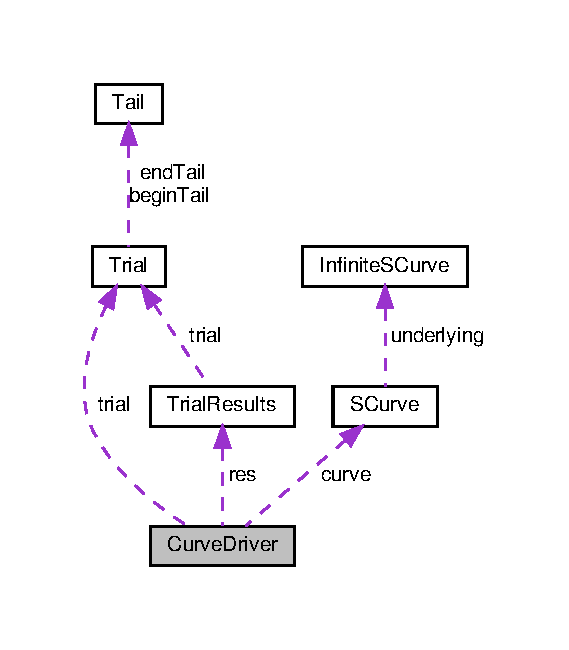
\includegraphics[width=273pt]{classCurveDriver__coll__graph}
\end{center}
\end{figure}
\subsection*{Public Member Functions}
\begin{DoxyCompactItemize}
\item 
\mbox{\Hypertarget{classCurveDriver_abd46031f6a7c1f4b5cc8c8ecb5dd25da}\label{classCurveDriver_abd46031f6a7c1f4b5cc8c8ecb5dd25da}} 
{\bfseries Curve\+Driver} (\hyperlink{structTrialResults}{Trial\+Results} \&itrial, okapi\+::\+Abstract\+Motor \&ioutput)
\item 
\mbox{\Hypertarget{classCurveDriver_a87ee8989aae5b597f1788de01de5a7eb}\label{classCurveDriver_a87ee8989aae5b597f1788de01de5a7eb}} 
double {\bfseries elapsed} ()
\item 
\mbox{\Hypertarget{classCurveDriver_a92ed2d7443067b2233cd24be086cbd7a}\label{classCurveDriver_a92ed2d7443067b2233cd24be086cbd7a}} 
double {\bfseries disp} ()
\item 
\mbox{\Hypertarget{classCurveDriver_acc6953f0a4221bc987b7f31c7f9e8a89}\label{classCurveDriver_acc6953f0a4221bc987b7f31c7f9e8a89}} 
double {\bfseries real\+Vel} ()
\item 
\mbox{\Hypertarget{classCurveDriver_acc2eadbd0a2788e6db0c21b39e136bbe}\label{classCurveDriver_acc2eadbd0a2788e6db0c21b39e136bbe}} 
double {\bfseries vel\+For\+Disp} (double d)
\item 
\mbox{\Hypertarget{classCurveDriver_a2932cc25ea69dd3dfb88a2790be84814}\label{classCurveDriver_a2932cc25ea69dd3dfb88a2790be84814}} 
void {\bfseries drive\+For\+Time} (double t)
\item 
\mbox{\Hypertarget{classCurveDriver_aa4f8ee1ee14a30829c473aa5299d9a8d}\label{classCurveDriver_aa4f8ee1ee14a30829c473aa5299d9a8d}} 
double {\bfseries predicted\+Time\+Remaining} ()
\end{DoxyCompactItemize}
\subsection*{Public Attributes}
\begin{DoxyCompactItemize}
\item 
\mbox{\Hypertarget{classCurveDriver_afa8957da40dcef07c00047f9a12f5320}\label{classCurveDriver_afa8957da40dcef07c00047f9a12f5320}} 
\hyperlink{structTrialResults}{Trial\+Results} \& {\bfseries res}
\item 
\mbox{\Hypertarget{classCurveDriver_a4712df5b8884fdd496fbd512c283d7c3}\label{classCurveDriver_a4712df5b8884fdd496fbd512c283d7c3}} 
\hyperlink{structTrial}{Trial} \& {\bfseries trial}
\item 
\mbox{\Hypertarget{classCurveDriver_af272be4d71737ca39590b591c472a7f5}\label{classCurveDriver_af272be4d71737ca39590b591c472a7f5}} 
\hyperlink{classSCurve}{S\+Curve} {\bfseries curve}
\item 
\mbox{\Hypertarget{classCurveDriver_a92a10c15098ba3e2aaa42738f9b0d165}\label{classCurveDriver_a92a10c15098ba3e2aaa42738f9b0d165}} 
std\+::vector$<$ \hyperlink{structPosition}{Position} $>$ \& {\bfseries data}
\item 
\mbox{\Hypertarget{classCurveDriver_a2ea2f4bf49841ec7e87c13bb57a48b45}\label{classCurveDriver_a2ea2f4bf49841ec7e87c13bb57a48b45}} 
okapi\+::\+Abstract\+Motor \& {\bfseries output}
\item 
\mbox{\Hypertarget{classCurveDriver_a5c474d5b677786a32b77f3d64af17487}\label{classCurveDriver_a5c474d5b677786a32b77f3d64af17487}} 
uint64\+\_\+t {\bfseries begin\+Time}
\item 
\mbox{\Hypertarget{classCurveDriver_ad923e6b468b113058348bc99d5f4527b}\label{classCurveDriver_ad923e6b468b113058348bc99d5f4527b}} 
double {\bfseries begin\+Reading}
\item 
\mbox{\Hypertarget{classCurveDriver_ad8441a570e2ed8fd33372ed3aa483412}\label{classCurveDriver_ad8441a570e2ed8fd33372ed3aa483412}} 
double {\bfseries last\+Used\+Time} = 0
\item 
\mbox{\Hypertarget{classCurveDriver_a257a08923ce5d9341577a1212259b523}\label{classCurveDriver_a257a08923ce5d9341577a1212259b523}} 
bool {\bfseries stop\+On\+Finish}
\item 
\mbox{\Hypertarget{classCurveDriver_a79818829bc9d403361ea7c108edbd110}\label{classCurveDriver_a79818829bc9d403361ea7c108edbd110}} 
okapi\+::\+Abstract\+Motor\+::brake\+Mode {\bfseries stop\+Brake\+Mode}
\end{DoxyCompactItemize}


The documentation for this class was generated from the following file\+:\begin{DoxyCompactItemize}
\item 
src/followtest.\+cpp\end{DoxyCompactItemize}

\hypertarget{classEncoderAverage}{}\section{Encoder\+Average Class Reference}
\label{classEncoderAverage}\index{Encoder\+Average@{Encoder\+Average}}


Inheritance diagram for Encoder\+Average\+:\nopagebreak
\begin{figure}[H]
\begin{center}
\leavevmode
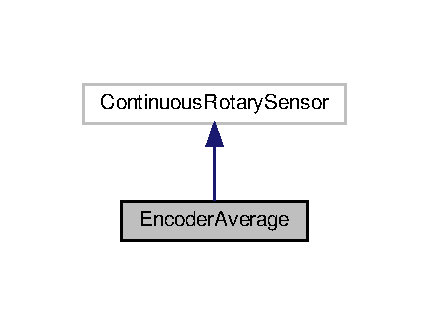
\includegraphics[width=206pt]{classEncoderAverage__inherit__graph}
\end{center}
\end{figure}


Collaboration diagram for Encoder\+Average\+:\nopagebreak
\begin{figure}[H]
\begin{center}
\leavevmode
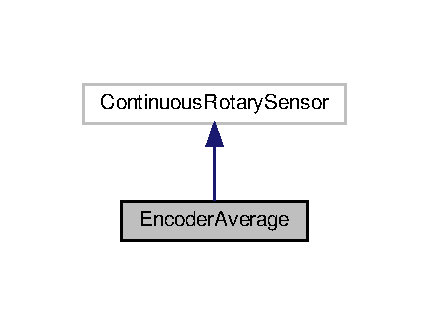
\includegraphics[width=206pt]{classEncoderAverage__coll__graph}
\end{center}
\end{figure}
\subsection*{Public Member Functions}
\begin{DoxyCompactItemize}
\item 
\mbox{\Hypertarget{classEncoderAverage_a724597f4db6dd249fbb4e1f7e2e72322}\label{classEncoderAverage_a724597f4db6dd249fbb4e1f7e2e72322}} 
{\bfseries Encoder\+Average} (std\+::initializer\+\_\+list$<$ std\+::shared\+\_\+ptr$<$ okapi\+::\+Continuous\+Rotary\+Sensor $>$$>$ sensors)
\item 
\mbox{\Hypertarget{classEncoderAverage_a5255c50e635177b4ff0589de299965d9}\label{classEncoderAverage_a5255c50e635177b4ff0589de299965d9}} 
double {\bfseries get} () const override
\item 
\mbox{\Hypertarget{classEncoderAverage_afe094e54cc09ea812602ad014c2287b0}\label{classEncoderAverage_afe094e54cc09ea812602ad014c2287b0}} 
double {\bfseries controller\+Get} () override
\item 
\mbox{\Hypertarget{classEncoderAverage_a3f5cb96c7f86a893d10ce6b6e5773ba8}\label{classEncoderAverage_a3f5cb96c7f86a893d10ce6b6e5773ba8}} 
std\+::int32\+\_\+t {\bfseries reset} () override
\end{DoxyCompactItemize}
\subsection*{Private Attributes}
\begin{DoxyCompactItemize}
\item 
\mbox{\Hypertarget{classEncoderAverage_a58663dbf442771f7e43fbb9ab3d7b902}\label{classEncoderAverage_a58663dbf442771f7e43fbb9ab3d7b902}} 
std\+::vector$<$ std\+::shared\+\_\+ptr$<$ okapi\+::\+Continuous\+Rotary\+Sensor $>$ $>$ {\bfseries my\+Sensors}
\end{DoxyCompactItemize}


The documentation for this class was generated from the following file\+:\begin{DoxyCompactItemize}
\item 
src/mtrs.\+hpp\end{DoxyCompactItemize}

\hypertarget{classExtraSpecialMotorWithExternalSensorsAsEncoders}{}\section{Extra\+Special\+Motor\+With\+External\+Sensors\+As\+Encoders Class Reference}
\label{classExtraSpecialMotorWithExternalSensorsAsEncoders}\index{Extra\+Special\+Motor\+With\+External\+Sensors\+As\+Encoders@{Extra\+Special\+Motor\+With\+External\+Sensors\+As\+Encoders}}


Inheritance diagram for Extra\+Special\+Motor\+With\+External\+Sensors\+As\+Encoders\+:\nopagebreak
\begin{figure}[H]
\begin{center}
\leavevmode
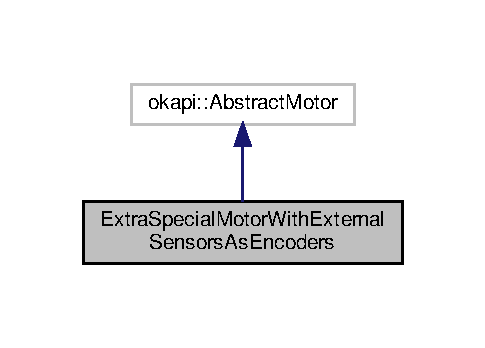
\includegraphics[width=233pt]{classExtraSpecialMotorWithExternalSensorsAsEncoders__inherit__graph}
\end{center}
\end{figure}


Collaboration diagram for Extra\+Special\+Motor\+With\+External\+Sensors\+As\+Encoders\+:\nopagebreak
\begin{figure}[H]
\begin{center}
\leavevmode
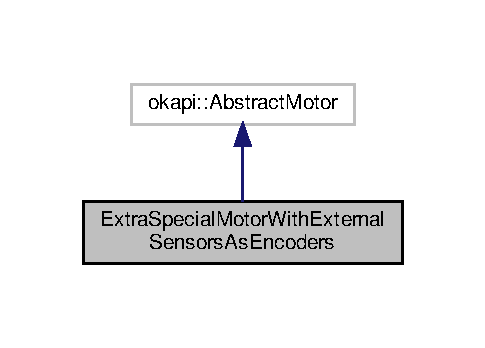
\includegraphics[width=233pt]{classExtraSpecialMotorWithExternalSensorsAsEncoders__coll__graph}
\end{center}
\end{figure}
\subsection*{Public Member Functions}
\begin{DoxyCompactItemize}
\item 
\mbox{\Hypertarget{classExtraSpecialMotorWithExternalSensorsAsEncoders_a3fb898c76f246c08d0634933fea4a557}\label{classExtraSpecialMotorWithExternalSensorsAsEncoders_a3fb898c76f246c08d0634933fea4a557}} 
{\bfseries Extra\+Special\+Motor\+With\+External\+Sensors\+As\+Encoders} (okapi\+::\+Abstract\+Motor \&icaptive, std\+::shared\+\_\+ptr$<$ okapi\+::\+Continuous\+Rotary\+Sensor $>$ ienc)
\item 
\mbox{\Hypertarget{classExtraSpecialMotorWithExternalSensorsAsEncoders_af77f0f3c65fa7e19fd49a25b86694597}\label{classExtraSpecialMotorWithExternalSensorsAsEncoders_af77f0f3c65fa7e19fd49a25b86694597}} 
std\+::int32\+\_\+t {\bfseries move\+Absolute} (double position, std\+::int32\+\_\+t velocity) override
\item 
\mbox{\Hypertarget{classExtraSpecialMotorWithExternalSensorsAsEncoders_a688e2df620b1c931c448041ef2728966}\label{classExtraSpecialMotorWithExternalSensorsAsEncoders_a688e2df620b1c931c448041ef2728966}} 
std\+::int32\+\_\+t {\bfseries move\+Relative} (double position, std\+::int32\+\_\+t velocity) override
\item 
\mbox{\Hypertarget{classExtraSpecialMotorWithExternalSensorsAsEncoders_ae1378301e9848847026f342df66f6762}\label{classExtraSpecialMotorWithExternalSensorsAsEncoders_ae1378301e9848847026f342df66f6762}} 
std\+::int32\+\_\+t {\bfseries move\+Velocity} (std\+::int16\+\_\+t velocity) override
\item 
\mbox{\Hypertarget{classExtraSpecialMotorWithExternalSensorsAsEncoders_a1dee79ad417eba651537ef56b32cd9c3}\label{classExtraSpecialMotorWithExternalSensorsAsEncoders_a1dee79ad417eba651537ef56b32cd9c3}} 
std\+::int32\+\_\+t {\bfseries move\+Voltage} (std\+::int16\+\_\+t voltage) override
\item 
\mbox{\Hypertarget{classExtraSpecialMotorWithExternalSensorsAsEncoders_a21482d2a303737d582961a90de113f62}\label{classExtraSpecialMotorWithExternalSensorsAsEncoders_a21482d2a303737d582961a90de113f62}} 
double {\bfseries get\+Target\+Position} () override
\item 
\mbox{\Hypertarget{classExtraSpecialMotorWithExternalSensorsAsEncoders_a9661e8aef759e8a7784ac0f4eeddb5df}\label{classExtraSpecialMotorWithExternalSensorsAsEncoders_a9661e8aef759e8a7784ac0f4eeddb5df}} 
double {\bfseries get\+Position} () override
\item 
\mbox{\Hypertarget{classExtraSpecialMotorWithExternalSensorsAsEncoders_ac8ae94a48e71696e45271332bb0564f4}\label{classExtraSpecialMotorWithExternalSensorsAsEncoders_ac8ae94a48e71696e45271332bb0564f4}} 
std\+::int32\+\_\+t {\bfseries tare\+Position} () override
\item 
\mbox{\Hypertarget{classExtraSpecialMotorWithExternalSensorsAsEncoders_ac18c9c1a64d65cf19ced73098bbdee64}\label{classExtraSpecialMotorWithExternalSensorsAsEncoders_ac18c9c1a64d65cf19ced73098bbdee64}} 
std\+::int32\+\_\+t {\bfseries get\+Raw\+Position} (std\+::uint32\+\_\+t $\ast$timestamp) override
\item 
\mbox{\Hypertarget{classExtraSpecialMotorWithExternalSensorsAsEncoders_a025c9c6a3599c81122777b8f1285a79c}\label{classExtraSpecialMotorWithExternalSensorsAsEncoders_a025c9c6a3599c81122777b8f1285a79c}} 
std\+::int32\+\_\+t {\bfseries get\+Target\+Velocity} () override
\item 
\mbox{\Hypertarget{classExtraSpecialMotorWithExternalSensorsAsEncoders_ae7eb26bcbfa90bdc4434d542ca84aa90}\label{classExtraSpecialMotorWithExternalSensorsAsEncoders_ae7eb26bcbfa90bdc4434d542ca84aa90}} 
double {\bfseries get\+Actual\+Velocity} () override
\item 
\mbox{\Hypertarget{classExtraSpecialMotorWithExternalSensorsAsEncoders_a4810135b2e15a432e38b8904f16835d7}\label{classExtraSpecialMotorWithExternalSensorsAsEncoders_a4810135b2e15a432e38b8904f16835d7}} 
std\+::int32\+\_\+t {\bfseries get\+Current\+Draw} () override
\item 
\mbox{\Hypertarget{classExtraSpecialMotorWithExternalSensorsAsEncoders_a226cbe38bdaa546f28875e87347f3d37}\label{classExtraSpecialMotorWithExternalSensorsAsEncoders_a226cbe38bdaa546f28875e87347f3d37}} 
std\+::int32\+\_\+t {\bfseries get\+Direction} () override
\item 
\mbox{\Hypertarget{classExtraSpecialMotorWithExternalSensorsAsEncoders_a4e92371152dac8c2fef12390f178b3d0}\label{classExtraSpecialMotorWithExternalSensorsAsEncoders_a4e92371152dac8c2fef12390f178b3d0}} 
double {\bfseries get\+Efficiency} () override
\item 
\mbox{\Hypertarget{classExtraSpecialMotorWithExternalSensorsAsEncoders_a1c7d3f8220af691d5fe36999046a67a9}\label{classExtraSpecialMotorWithExternalSensorsAsEncoders_a1c7d3f8220af691d5fe36999046a67a9}} 
std\+::int32\+\_\+t {\bfseries is\+Over\+Current} () override
\item 
\mbox{\Hypertarget{classExtraSpecialMotorWithExternalSensorsAsEncoders_a5451be6b86b5f1e83f00593fbda10e41}\label{classExtraSpecialMotorWithExternalSensorsAsEncoders_a5451be6b86b5f1e83f00593fbda10e41}} 
std\+::int32\+\_\+t {\bfseries is\+Over\+Temp} () override
\item 
\mbox{\Hypertarget{classExtraSpecialMotorWithExternalSensorsAsEncoders_a7a954b681a8da95860b6904cc2646c5b}\label{classExtraSpecialMotorWithExternalSensorsAsEncoders_a7a954b681a8da95860b6904cc2646c5b}} 
std\+::int32\+\_\+t {\bfseries is\+Stopped} () override
\item 
\mbox{\Hypertarget{classExtraSpecialMotorWithExternalSensorsAsEncoders_a8de84376bb04415bcd0568f2318df63b}\label{classExtraSpecialMotorWithExternalSensorsAsEncoders_a8de84376bb04415bcd0568f2318df63b}} 
std\+::int32\+\_\+t {\bfseries get\+Zero\+Position\+Flag} () override
\item 
\mbox{\Hypertarget{classExtraSpecialMotorWithExternalSensorsAsEncoders_ae58b43f866abc93e8a4acff736736174}\label{classExtraSpecialMotorWithExternalSensorsAsEncoders_ae58b43f866abc93e8a4acff736736174}} 
uint32\+\_\+t {\bfseries get\+Faults} () override
\item 
\mbox{\Hypertarget{classExtraSpecialMotorWithExternalSensorsAsEncoders_a7e9836496884b7770c0fe7f2201d4790}\label{classExtraSpecialMotorWithExternalSensorsAsEncoders_a7e9836496884b7770c0fe7f2201d4790}} 
uint32\+\_\+t {\bfseries get\+Flags} () override
\item 
\mbox{\Hypertarget{classExtraSpecialMotorWithExternalSensorsAsEncoders_a596648a16cef504f164ba15f38d3dfc1}\label{classExtraSpecialMotorWithExternalSensorsAsEncoders_a596648a16cef504f164ba15f38d3dfc1}} 
double {\bfseries get\+Power} () override
\item 
\mbox{\Hypertarget{classExtraSpecialMotorWithExternalSensorsAsEncoders_a4efb4d364485b9f6c1553cf90b18416b}\label{classExtraSpecialMotorWithExternalSensorsAsEncoders_a4efb4d364485b9f6c1553cf90b18416b}} 
double {\bfseries get\+Temperature} () override
\item 
\mbox{\Hypertarget{classExtraSpecialMotorWithExternalSensorsAsEncoders_af34c4b8ce32c0abac0b064b868f1c490}\label{classExtraSpecialMotorWithExternalSensorsAsEncoders_af34c4b8ce32c0abac0b064b868f1c490}} 
double {\bfseries get\+Torque} () override
\item 
\mbox{\Hypertarget{classExtraSpecialMotorWithExternalSensorsAsEncoders_ab94b2c1489a5573a0ce8c86c89f93317}\label{classExtraSpecialMotorWithExternalSensorsAsEncoders_ab94b2c1489a5573a0ce8c86c89f93317}} 
std\+::int32\+\_\+t {\bfseries get\+Voltage} () override
\item 
\mbox{\Hypertarget{classExtraSpecialMotorWithExternalSensorsAsEncoders_ab98e930d87f2fee87828e94912b9f50a}\label{classExtraSpecialMotorWithExternalSensorsAsEncoders_ab98e930d87f2fee87828e94912b9f50a}} 
std\+::int32\+\_\+t {\bfseries set\+Brake\+Mode} (okapi\+::\+Abstract\+Motor\+::brake\+Mode b) override
\item 
\mbox{\Hypertarget{classExtraSpecialMotorWithExternalSensorsAsEncoders_a7dae127bac39f70638faf16aa17ebf9b}\label{classExtraSpecialMotorWithExternalSensorsAsEncoders_a7dae127bac39f70638faf16aa17ebf9b}} 
okapi\+::\+Abstract\+Motor\+::brake\+Mode {\bfseries get\+Brake\+Mode} () override
\item 
\mbox{\Hypertarget{classExtraSpecialMotorWithExternalSensorsAsEncoders_a90b9d8f7cb21519f93673cf415d16a8b}\label{classExtraSpecialMotorWithExternalSensorsAsEncoders_a90b9d8f7cb21519f93673cf415d16a8b}} 
std\+::int32\+\_\+t {\bfseries set\+Current\+Limit} (std\+::int32\+\_\+t limit) override
\item 
\mbox{\Hypertarget{classExtraSpecialMotorWithExternalSensorsAsEncoders_a063f36c30acb523dd1255284ba5ec47a}\label{classExtraSpecialMotorWithExternalSensorsAsEncoders_a063f36c30acb523dd1255284ba5ec47a}} 
std\+::int32\+\_\+t {\bfseries get\+Current\+Limit} () override
\item 
\mbox{\Hypertarget{classExtraSpecialMotorWithExternalSensorsAsEncoders_aa7573abc560785614b71662424ebf638}\label{classExtraSpecialMotorWithExternalSensorsAsEncoders_aa7573abc560785614b71662424ebf638}} 
std\+::int32\+\_\+t {\bfseries modify\+Profiled\+Velocity} (std\+::int32\+\_\+t vel) override
\item 
\mbox{\Hypertarget{classExtraSpecialMotorWithExternalSensorsAsEncoders_a165795fb85bd0542793469d6f6ed0a0b}\label{classExtraSpecialMotorWithExternalSensorsAsEncoders_a165795fb85bd0542793469d6f6ed0a0b}} 
double {\bfseries enc\+Gearing} ()
\item 
\mbox{\Hypertarget{classExtraSpecialMotorWithExternalSensorsAsEncoders_a08ec684e25bc9a79fcebff57f3792f0f}\label{classExtraSpecialMotorWithExternalSensorsAsEncoders_a08ec684e25bc9a79fcebff57f3792f0f}} 
std\+::int32\+\_\+t {\bfseries set\+Encoder\+Units} (okapi\+::\+Abstract\+Motor\+::encoder\+Units eunits) override
\item 
\mbox{\Hypertarget{classExtraSpecialMotorWithExternalSensorsAsEncoders_ac223ecd0ded6cdab47027da22ba9820e}\label{classExtraSpecialMotorWithExternalSensorsAsEncoders_ac223ecd0ded6cdab47027da22ba9820e}} 
okapi\+::\+Abstract\+Motor\+::encoder\+Units {\bfseries get\+Encoder\+Units} () override
\item 
\mbox{\Hypertarget{classExtraSpecialMotorWithExternalSensorsAsEncoders_a9bb9076765a1d8a346b4e4d9bec0f06d}\label{classExtraSpecialMotorWithExternalSensorsAsEncoders_a9bb9076765a1d8a346b4e4d9bec0f06d}} 
std\+::int32\+\_\+t {\bfseries set\+Gearing} (okapi\+::\+Abstract\+Motor\+::gearset gearing)
\item 
\mbox{\Hypertarget{classExtraSpecialMotorWithExternalSensorsAsEncoders_a60073af076a7e168da6ad4912b7eb7b5}\label{classExtraSpecialMotorWithExternalSensorsAsEncoders_a60073af076a7e168da6ad4912b7eb7b5}} 
okapi\+::\+Abstract\+Motor\+::gearset {\bfseries get\+Gearing} ()
\item 
\mbox{\Hypertarget{classExtraSpecialMotorWithExternalSensorsAsEncoders_aac68d3e2998d7200b405770d87b2538b}\label{classExtraSpecialMotorWithExternalSensorsAsEncoders_aac68d3e2998d7200b405770d87b2538b}} 
void {\bfseries set\+Enc\+Reversed} (bool is\+Reversed)
\item 
\mbox{\Hypertarget{classExtraSpecialMotorWithExternalSensorsAsEncoders_a43070ed9fe14fa70a8b7ba886385d7f1}\label{classExtraSpecialMotorWithExternalSensorsAsEncoders_a43070ed9fe14fa70a8b7ba886385d7f1}} 
std\+::int32\+\_\+t {\bfseries set\+Reversed} (bool is\+Reversed) override
\item 
\mbox{\Hypertarget{classExtraSpecialMotorWithExternalSensorsAsEncoders_a9ba712a6d09f2c4e5c88a300ff7da8ae}\label{classExtraSpecialMotorWithExternalSensorsAsEncoders_a9ba712a6d09f2c4e5c88a300ff7da8ae}} 
std\+::int32\+\_\+t {\bfseries set\+Voltage\+Limit} (std\+::int32\+\_\+t ilimit) override
\item 
\mbox{\Hypertarget{classExtraSpecialMotorWithExternalSensorsAsEncoders_ad27c1889e5a973795c41625b849f7259}\label{classExtraSpecialMotorWithExternalSensorsAsEncoders_ad27c1889e5a973795c41625b849f7259}} 
std\+::shared\+\_\+ptr$<$ okapi\+::\+Continuous\+Rotary\+Sensor $>$ {\bfseries get\+Encoder} () override
\item 
\mbox{\Hypertarget{classExtraSpecialMotorWithExternalSensorsAsEncoders_a9fd9f2baa1066023a25a62a2415857e5}\label{classExtraSpecialMotorWithExternalSensorsAsEncoders_a9fd9f2baa1066023a25a62a2415857e5}} 
void {\bfseries controller\+Set} (double vel)
\end{DoxyCompactItemize}
\subsection*{Private Attributes}
\begin{DoxyCompactItemize}
\item 
\mbox{\Hypertarget{classExtraSpecialMotorWithExternalSensorsAsEncoders_a6dddf188f2a1a4d2eec58f3948ef2e2f}\label{classExtraSpecialMotorWithExternalSensorsAsEncoders_a6dddf188f2a1a4d2eec58f3948ef2e2f}} 
okapi\+::\+Abstract\+Motor \& {\bfseries captive}
\item 
\mbox{\Hypertarget{classExtraSpecialMotorWithExternalSensorsAsEncoders_a349485b170fc2662123ff4c535876c67}\label{classExtraSpecialMotorWithExternalSensorsAsEncoders_a349485b170fc2662123ff4c535876c67}} 
std\+::shared\+\_\+ptr$<$ okapi\+::\+Continuous\+Rotary\+Sensor $>$ {\bfseries real\+Enc}
\item 
\mbox{\Hypertarget{classExtraSpecialMotorWithExternalSensorsAsEncoders_af2e13009e8d6e7b9a4b38e855aa778e7}\label{classExtraSpecialMotorWithExternalSensorsAsEncoders_af2e13009e8d6e7b9a4b38e855aa778e7}} 
double {\bfseries last\+Target} = 0
\item 
\mbox{\Hypertarget{classExtraSpecialMotorWithExternalSensorsAsEncoders_aa65162508dc977a0e242f7407b3e049b}\label{classExtraSpecialMotorWithExternalSensorsAsEncoders_aa65162508dc977a0e242f7407b3e049b}} 
double {\bfseries offset}
\item 
\mbox{\Hypertarget{classExtraSpecialMotorWithExternalSensorsAsEncoders_a5550247e91f7881a790c0bac418101db}\label{classExtraSpecialMotorWithExternalSensorsAsEncoders_a5550247e91f7881a790c0bac418101db}} 
double {\bfseries units} = 1
\end{DoxyCompactItemize}


The documentation for this class was generated from the following file\+:\begin{DoxyCompactItemize}
\item 
src/mtrs.\+hpp\end{DoxyCompactItemize}

\hypertarget{structInfiniteSCurve}{}\section{Infinite\+S\+Curve Struct Reference}
\label{structInfiniteSCurve}\index{Infinite\+S\+Curve@{Infinite\+S\+Curve}}
\subsection*{Public Member Functions}
\begin{DoxyCompactItemize}
\item 
\mbox{\Hypertarget{structInfiniteSCurve_aceefa8b485ba846876810080694c8161}\label{structInfiniteSCurve_aceefa8b485ba846876810080694c8161}} 
double {\bfseries calc\+Fwd\+Jerk\+Limit} (double time)
\item 
\mbox{\Hypertarget{structInfiniteSCurve_a8741f0b3363ec756bb5e1354241ae547}\label{structInfiniteSCurve_a8741f0b3363ec756bb5e1354241ae547}} 
double {\bfseries calc\+Rev\+Jerk\+Limit} (double time)
\item 
\mbox{\Hypertarget{structInfiniteSCurve_a351be64405faf57e20810a59f0ee2a10}\label{structInfiniteSCurve_a351be64405faf57e20810a59f0ee2a10}} 
double {\bfseries calc\+Acc\+Limit} (double time)
\item 
\mbox{\Hypertarget{structInfiniteSCurve_abdc923945779b11a417ced169c9d79aa}\label{structInfiniteSCurve_abdc923945779b11a417ced169c9d79aa}} 
{\bfseries Infinite\+S\+Curve} (double v, double a, double j)
\item 
\mbox{\Hypertarget{structInfiniteSCurve_a224dd310c22430f53bae464479449b0c}\label{structInfiniteSCurve_a224dd310c22430f53bae464479449b0c}} 
double {\bfseries calc} (double num)
\item 
\mbox{\Hypertarget{structInfiniteSCurve_a1d0d395b4f5ed515c6e62b91c837dafa}\label{structInfiniteSCurve_a1d0d395b4f5ed515c6e62b91c837dafa}} 
double {\bfseries calc\+Time\+For\+Pos} (double pos)
\item 
\mbox{\Hypertarget{structInfiniteSCurve_a109574e9697b2ce83961889898f6425e}\label{structInfiniteSCurve_a109574e9697b2ce83961889898f6425e}} 
double {\bfseries calc\+Pos\+For\+Time} (double time)
\item 
\mbox{\Hypertarget{structInfiniteSCurve_a6525ffc67eb4568b9a27d9555172a973}\label{structInfiniteSCurve_a6525ffc67eb4568b9a27d9555172a973}} 
double {\bfseries calc\+Acc\+For\+Time} (double time)
\item 
\mbox{\Hypertarget{structInfiniteSCurve_a1b295c1675d6295a13badbd0e39dfc58}\label{structInfiniteSCurve_a1b295c1675d6295a13badbd0e39dfc58}} 
double {\bfseries min\+Pos} ()
\item 
\mbox{\Hypertarget{structInfiniteSCurve_a03647e0572ea4399038316e85e0e9eab}\label{structInfiniteSCurve_a03647e0572ea4399038316e85e0e9eab}} 
double {\bfseries min\+Half\+Width} ()
\end{DoxyCompactItemize}
\subsection*{Public Attributes}
\begin{DoxyCompactItemize}
\item 
\mbox{\Hypertarget{structInfiniteSCurve_afffeea3c29edeb6f435d56d0890bfc24}\label{structInfiniteSCurve_afffeea3c29edeb6f435d56d0890bfc24}} 
double {\bfseries vel\+Limit}
\item 
\mbox{\Hypertarget{structInfiniteSCurve_a9a88861b36039656051de878c7dd0a49}\label{structInfiniteSCurve_a9a88861b36039656051de878c7dd0a49}} 
double {\bfseries acc\+Limit}
\item 
\mbox{\Hypertarget{structInfiniteSCurve_a003a161d42ef0fa689a6b14dee4893b8}\label{structInfiniteSCurve_a003a161d42ef0fa689a6b14dee4893b8}} 
double {\bfseries jrk\+Limit}
\item 
\mbox{\Hypertarget{structInfiniteSCurve_a853f84ab263de53a283e87c466b55500}\label{structInfiniteSCurve_a853f84ab263de53a283e87c466b55500}} 
bool {\bfseries has\+An\+Acc\+Limiter} = true
\item 
\mbox{\Hypertarget{structInfiniteSCurve_a5bf95b93d8fc8fd523834d9c4f0dd30b}\label{structInfiniteSCurve_a5bf95b93d8fc8fd523834d9c4f0dd30b}} 
std\+::vector$<$ \hyperlink{structSlice}{Slice} $>$ {\bfseries slices}
\end{DoxyCompactItemize}


The documentation for this struct was generated from the following file\+:\begin{DoxyCompactItemize}
\item 
src/scurve.\+hpp\end{DoxyCompactItemize}

\hypertarget{structMessage}{}\section{Message Struct Reference}
\label{structMessage}\index{Message@{Message}}
\subsection*{Public Member Functions}
\begin{DoxyCompactItemize}
\item 
\mbox{\Hypertarget{structMessage_a5a9039f0cad6557ac75812d25be50ac8}\label{structMessage_a5a9039f0cad6557ac75812d25be50ac8}} 
{\bfseries Message} (const std\+::string \&text)
\item 
\mbox{\Hypertarget{structMessage_a7e93ac9c9e381104189a00b7aabdb1d5}\label{structMessage_a7e93ac9c9e381104189a00b7aabdb1d5}} 
std\+::string {\bfseries text} ()
\item 
\mbox{\Hypertarget{structMessage_a6d29dfff8b2c60ad5e1607e406ab16ae}\label{structMessage_a6d29dfff8b2c60ad5e1607e406ab16ae}} 
void {\bfseries send} ()
\item 
\mbox{\Hypertarget{structMessage_a508c02bc99ad9ce50e126f7d32631be2}\label{structMessage_a508c02bc99ad9ce50e126f7d32631be2}} 
void {\bfseries big\+Send} ()
\item 
\mbox{\Hypertarget{structMessage_a38316155aff71ea12fc3f66a1a463ab0}\label{structMessage_a38316155aff71ea12fc3f66a1a463ab0}} 
double {\bfseries number} (const std\+::string \&key) const
\item 
\mbox{\Hypertarget{structMessage_a1651453c7fa6cbe6676adab451025a32}\label{structMessage_a1651453c7fa6cbe6676adab451025a32}} 
int {\bfseries integer} (const std\+::string \&key) const
\item 
\mbox{\Hypertarget{structMessage_a69fad2186f7767460e1e6758b3090dc0}\label{structMessage_a69fad2186f7767460e1e6758b3090dc0}} 
std\+::string {\bfseries string} (const std\+::string \&key) const
\item 
\mbox{\Hypertarget{structMessage_a7cb4297d790407676b91edd8652e400a}\label{structMessage_a7cb4297d790407676b91edd8652e400a}} 
bool {\bfseries boolean} (const std\+::string \&key) const
\end{DoxyCompactItemize}
\subsection*{Public Attributes}
\begin{DoxyCompactItemize}
\item 
\mbox{\Hypertarget{structMessage_a68f6134fbd3f9ee60933b795736ee48c}\label{structMessage_a68f6134fbd3f9ee60933b795736ee48c}} 
Address\+Kind {\bfseries address\+Kind}
\item 
\mbox{\Hypertarget{structMessage_af327f99cff6a93dd35c9205b026c5286}\label{structMessage_af327f99cff6a93dd35c9205b026c5286}} 
std\+::string {\bfseries address}
\item 
\mbox{\Hypertarget{structMessage_a5883e8b2fa30ad34978871f392ba36c3}\label{structMessage_a5883e8b2fa30ad34978871f392ba36c3}} 
std\+::string {\bfseries id}
\item 
\mbox{\Hypertarget{structMessage_a5e31a45b322f0d84a62a87a88243d728}\label{structMessage_a5e31a45b322f0d84a62a87a88243d728}} 
json {\bfseries content}
\end{DoxyCompactItemize}


The documentation for this struct was generated from the following files\+:\begin{DoxyCompactItemize}
\item 
src/tabu.\+hpp\item 
src/tabu.\+cpp\end{DoxyCompactItemize}

\hypertarget{structMotors}{}\section{Motors Struct Reference}
\label{structMotors}\index{Motors@{Motors}}
\subsection*{Public Attributes}
\begin{DoxyCompactItemize}
\item 
\mbox{\Hypertarget{structMotors_a5d90605286ca0f8c23b6028ac8effa99}\label{structMotors_a5d90605286ca0f8c23b6028ac8effa99}} 
okapi\+::\+Motor\+Group {\bfseries left} \{ 7, 9\}
\item 
\mbox{\Hypertarget{structMotors_aace6e441817be571ca0b47544651524c}\label{structMotors_aace6e441817be571ca0b47544651524c}} 
okapi\+::\+Motor\+Group {\bfseries right} \{-\/ 1, -\/ 2\}
\item 
\mbox{\Hypertarget{structMotors_a0db996aa93ee6158ae31e1a731f7cab2}\label{structMotors_a0db996aa93ee6158ae31e1a731f7cab2}} 
okapi\+::\+Motor\+Group {\bfseries all} \{ 7, 9, -\/ 1, -\/ 2\}
\item 
\mbox{\Hypertarget{structMotors_a078d4438849e9932901729f486d2d81d}\label{structMotors_a078d4438849e9932901729f486d2d81d}} 
okapi\+::\+Motor\+Group {\bfseries turn} \{ 7, 9, 1, 2\}
\item 
\mbox{\Hypertarget{structMotors_a72cd7862603c24e3fafd849f76035935}\label{structMotors_a72cd7862603c24e3fafd849f76035935}} 
okapi\+::\+Motor\+Group {\bfseries intake} \{ 20, -\/11\}
\item 
\mbox{\Hypertarget{structMotors_a60bfc869c3283289d502741a39b74d83}\label{structMotors_a60bfc869c3283289d502741a39b74d83}} 
okapi\+::\+Motor\+Group {\bfseries tilter} \{ 3\}
\item 
\mbox{\Hypertarget{structMotors_a2bff81f52c0339b7c92cdfa0827f7b6c}\label{structMotors_a2bff81f52c0339b7c92cdfa0827f7b6c}} 
okapi\+::\+Motor\+Group {\bfseries lift} \{ 8\}
\end{DoxyCompactItemize}


The documentation for this struct was generated from the following file\+:\begin{DoxyCompactItemize}
\item 
src/mtrs.\+hpp\end{DoxyCompactItemize}

\hypertarget{structPIDDataPoint}{}\section{P\+I\+D\+Data\+Point Struct Reference}
\label{structPIDDataPoint}\index{P\+I\+D\+Data\+Point@{P\+I\+D\+Data\+Point}}
\subsection*{Public Attributes}
\begin{DoxyCompactItemize}
\item 
\mbox{\Hypertarget{structPIDDataPoint_a187b5e81e75466a827535883d32cf58c}\label{structPIDDataPoint_a187b5e81e75466a827535883d32cf58c}} 
double {\bfseries time}
\item 
\mbox{\Hypertarget{structPIDDataPoint_a7d21cd9e9767da2c07176780eafb7f9f}\label{structPIDDataPoint_a7d21cd9e9767da2c07176780eafb7f9f}} 
double {\bfseries error}
\item 
\mbox{\Hypertarget{structPIDDataPoint_af786ef7b26e1fc20603ab026b0d828b0}\label{structPIDDataPoint_af786ef7b26e1fc20603ab026b0d828b0}} 
double {\bfseries p}
\item 
\mbox{\Hypertarget{structPIDDataPoint_ab394291471c2941ba60c6b061f3801ff}\label{structPIDDataPoint_ab394291471c2941ba60c6b061f3801ff}} 
double {\bfseries i}
\item 
\mbox{\Hypertarget{structPIDDataPoint_a074a6d224d88f3926a7542dbd235284b}\label{structPIDDataPoint_a074a6d224d88f3926a7542dbd235284b}} 
double {\bfseries d}
\item 
\mbox{\Hypertarget{structPIDDataPoint_a44d10198278ca28699d86d65810252c3}\label{structPIDDataPoint_a44d10198278ca28699d86d65810252c3}} 
double {\bfseries step}
\end{DoxyCompactItemize}


The documentation for this struct was generated from the following file\+:\begin{DoxyCompactItemize}
\item 
src/pidtest.\+cpp\end{DoxyCompactItemize}

\hypertarget{structPosition}{}\section{Position Struct Reference}
\label{structPosition}\index{Position@{Position}}
\subsection*{Public Attributes}
\begin{DoxyCompactItemize}
\item 
\mbox{\Hypertarget{structPosition_aca65d81e8c3f50786365ac22c4e077bd}\label{structPosition_aca65d81e8c3f50786365ac22c4e077bd}} 
double {\bfseries time}
\item 
\mbox{\Hypertarget{structPosition_a06b75a533b23e3814633aeea8858e71f}\label{structPosition_a06b75a533b23e3814633aeea8858e71f}} 
double {\bfseries disp}
\item 
\mbox{\Hypertarget{structPosition_a5ec27ede6fe004c00c2a78732cd7d658}\label{structPosition_a5ec27ede6fe004c00c2a78732cd7d658}} 
double {\bfseries c\+Vel}
\item 
\mbox{\Hypertarget{structPosition_ab257e5d4c700b3fcb782d84b67b11a07}\label{structPosition_ab257e5d4c700b3fcb782d84b67b11a07}} 
double {\bfseries m\+Vel}
\item 
\mbox{\Hypertarget{structPosition_a3c67162c41350e3efac3f062dfa5da92}\label{structPosition_a3c67162c41350e3efac3f062dfa5da92}} 
double {\bfseries d\+Vel}
\end{DoxyCompactItemize}


The documentation for this struct was generated from the following file\+:\begin{DoxyCompactItemize}
\item 
src/followtest.\+cpp\end{DoxyCompactItemize}

\hypertarget{classReversedEncoder}{}\section{Reversed\+Encoder Class Reference}
\label{classReversedEncoder}\index{Reversed\+Encoder@{Reversed\+Encoder}}


Inheritance diagram for Reversed\+Encoder\+:\nopagebreak
\begin{figure}[H]
\begin{center}
\leavevmode
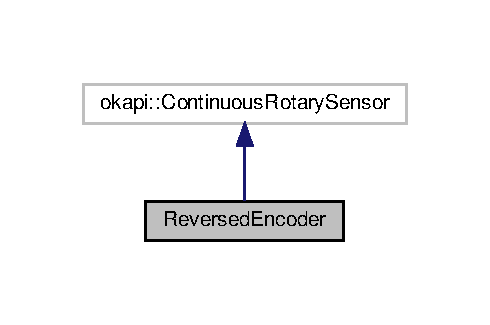
\includegraphics[width=235pt]{classReversedEncoder__inherit__graph}
\end{center}
\end{figure}


Collaboration diagram for Reversed\+Encoder\+:\nopagebreak
\begin{figure}[H]
\begin{center}
\leavevmode
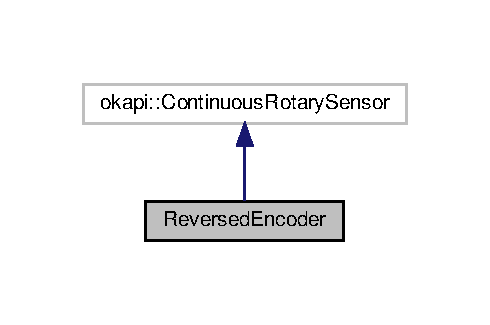
\includegraphics[width=235pt]{classReversedEncoder__coll__graph}
\end{center}
\end{figure}
\subsection*{Public Member Functions}
\begin{DoxyCompactItemize}
\item 
\mbox{\Hypertarget{classReversedEncoder_a06e957ec803cac9964921f19d003fa43}\label{classReversedEncoder_a06e957ec803cac9964921f19d003fa43}} 
{\bfseries Reversed\+Encoder} (std\+::shared\+\_\+ptr$<$ okapi\+::\+Continuous\+Rotary\+Sensor $>$ sensor)
\item 
\mbox{\Hypertarget{classReversedEncoder_a528b2fd3d24d1a68a6374d9e957315b3}\label{classReversedEncoder_a528b2fd3d24d1a68a6374d9e957315b3}} 
double {\bfseries get} () const override
\item 
\mbox{\Hypertarget{classReversedEncoder_a3b33e15d1282f03e6adf3cbbaf81d1d1}\label{classReversedEncoder_a3b33e15d1282f03e6adf3cbbaf81d1d1}} 
double {\bfseries controller\+Get} () override
\item 
\mbox{\Hypertarget{classReversedEncoder_ae13ab8af5aebbb48a09ed63ce7bdfeaa}\label{classReversedEncoder_ae13ab8af5aebbb48a09ed63ce7bdfeaa}} 
std\+::int32\+\_\+t {\bfseries reset} () override
\end{DoxyCompactItemize}
\subsection*{Private Attributes}
\begin{DoxyCompactItemize}
\item 
\mbox{\Hypertarget{classReversedEncoder_a8b176cecab772e61977b1b733e77d5c9}\label{classReversedEncoder_a8b176cecab772e61977b1b733e77d5c9}} 
std\+::shared\+\_\+ptr$<$ okapi\+::\+Continuous\+Rotary\+Sensor $>$ {\bfseries encoder}
\end{DoxyCompactItemize}


The documentation for this class was generated from the following file\+:\begin{DoxyCompactItemize}
\item 
src/mtrs.\+hpp\end{DoxyCompactItemize}

\hypertarget{classSCurve}{}\section{S\+Curve Class Reference}
\label{classSCurve}\index{S\+Curve@{S\+Curve}}


Collaboration diagram for S\+Curve\+:\nopagebreak
\begin{figure}[H]
\begin{center}
\leavevmode
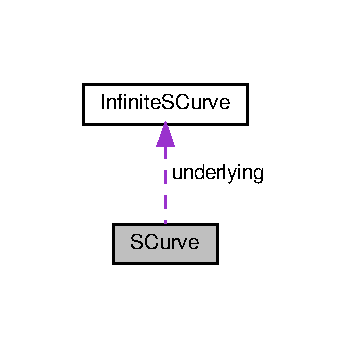
\includegraphics[width=168pt]{classSCurve__coll__graph}
\end{center}
\end{figure}
\subsection*{Public Member Functions}
\begin{DoxyCompactItemize}
\item 
\mbox{\Hypertarget{classSCurve_a3e399a2be395460823476a4f2d881fff}\label{classSCurve_a3e399a2be395460823476a4f2d881fff}} 
{\bfseries S\+Curve} (double v, double a, double j, double d)
\item 
\mbox{\Hypertarget{classSCurve_a34f5a1a56854e9297fddfa07c422e974}\label{classSCurve_a34f5a1a56854e9297fddfa07c422e974}} 
double {\bfseries calc} (double num)
\item 
\mbox{\Hypertarget{classSCurve_a332bc29667ae14b150d16388027cff9a}\label{classSCurve_a332bc29667ae14b150d16388027cff9a}} 
double {\bfseries calc\+Pos\+For\+Time} (double num)
\item 
\mbox{\Hypertarget{classSCurve_a167555657b6d99e26c3538a715a14de6}\label{classSCurve_a167555657b6d99e26c3538a715a14de6}} 
double {\bfseries calc\+Acc\+For\+Time} (double num)
\item 
\mbox{\Hypertarget{classSCurve_aad5d2c65fbee40f77d28529854c05e88}\label{classSCurve_aad5d2c65fbee40f77d28529854c05e88}} 
double {\bfseries calc\+Time\+For\+Pos} (double pos)
\item 
\mbox{\Hypertarget{classSCurve_ac1b45b15d7d29a863de7d11583ed3afb}\label{classSCurve_ac1b45b15d7d29a863de7d11583ed3afb}} 
double {\bfseries timing\+Width} ()
\end{DoxyCompactItemize}
\subsection*{Public Attributes}
\begin{DoxyCompactItemize}
\item 
\mbox{\Hypertarget{classSCurve_ac886cfc41a724e4218f544ab6c360359}\label{classSCurve_ac886cfc41a724e4218f544ab6c360359}} 
\hyperlink{structInfiniteSCurve}{Infinite\+S\+Curve} {\bfseries underlying}
\item 
\mbox{\Hypertarget{classSCurve_a5614565910af8581fa3806b3c8337eb9}\label{classSCurve_a5614565910af8581fa3806b3c8337eb9}} 
const double {\bfseries vel\+Limit}
\item 
\mbox{\Hypertarget{classSCurve_a24efc2a4fc25ad5744a6880f82d8f45e}\label{classSCurve_a24efc2a4fc25ad5744a6880f82d8f45e}} 
const double {\bfseries acc\+Limit}
\item 
\mbox{\Hypertarget{classSCurve_a7581bae615cbf086aaf01fe2f0276e6d}\label{classSCurve_a7581bae615cbf086aaf01fe2f0276e6d}} 
const double {\bfseries jrk\+Limit}
\item 
\mbox{\Hypertarget{classSCurve_a16296957d5dfb480cffd47b96a211789}\label{classSCurve_a16296957d5dfb480cffd47b96a211789}} 
const double {\bfseries distance}
\item 
\mbox{\Hypertarget{classSCurve_aaabc0d38585486ef01eee4d36e929772}\label{classSCurve_aaabc0d38585486ef01eee4d36e929772}} 
double {\bfseries t\+Width}
\end{DoxyCompactItemize}


The documentation for this class was generated from the following file\+:\begin{DoxyCompactItemize}
\item 
src/scurve.\+hpp\end{DoxyCompactItemize}

\hypertarget{structSlice}{}\section{Slice Struct Reference}
\label{structSlice}\index{Slice@{Slice}}
\subsection*{Public Attributes}
\begin{DoxyCompactItemize}
\item 
\mbox{\Hypertarget{structSlice_adfcca7658989ebb2c0faf1148813709c}\label{structSlice_adfcca7658989ebb2c0faf1148813709c}} 
double {\bfseries end\+Time}
\item 
\mbox{\Hypertarget{structSlice_ae012273ef688ac6d5333f48f385a0b0c}\label{structSlice_ae012273ef688ac6d5333f48f385a0b0c}} 
double {\bfseries y\+Translation\+Next}
\item 
\mbox{\Hypertarget{structSlice_a3ada29863e849be4433e63c832353f36}\label{structSlice_a3ada29863e849be4433e63c832353f36}} 
double {\bfseries def\+Integral}
\end{DoxyCompactItemize}


The documentation for this struct was generated from the following file\+:\begin{DoxyCompactItemize}
\item 
src/scurve.\+hpp\end{DoxyCompactItemize}

\hypertarget{classTabuLock}{}\section{Tabu\+Lock Class Reference}
\label{classTabuLock}\index{Tabu\+Lock@{Tabu\+Lock}}
\subsection*{Public Member Functions}
\begin{DoxyCompactItemize}
\item 
\mbox{\Hypertarget{classTabuLock_abe8c5cb1f343a72d0cdac3ee6f917c22}\label{classTabuLock_abe8c5cb1f343a72d0cdac3ee6f917c22}} 
void {\bfseries give} ()
\item 
\mbox{\Hypertarget{classTabuLock_a6f6308ba394ad0067611d6b8b154a323}\label{classTabuLock_a6f6308ba394ad0067611d6b8b154a323}} 
void {\bfseries take} ()
\end{DoxyCompactItemize}
\subsection*{Private Attributes}
\begin{DoxyCompactItemize}
\item 
\mbox{\Hypertarget{classTabuLock_a6977b5fa71b91ac9aa65be746c607ed4}\label{classTabuLock_a6977b5fa71b91ac9aa65be746c607ed4}} 
bool {\bfseries taken} = false
\end{DoxyCompactItemize}


The documentation for this class was generated from the following file\+:\begin{DoxyCompactItemize}
\item 
src/tabu.\+cpp\end{DoxyCompactItemize}

\hypertarget{structTail}{}\section{Tail Struct Reference}
\label{structTail}\index{Tail@{Tail}}
\subsection*{Public Member Functions}
\begin{DoxyCompactItemize}
\item 
\mbox{\Hypertarget{structTail_a44f3d1d2a4273e2c5c15e1c98a2c4117}\label{structTail_a44f3d1d2a4273e2c5c15e1c98a2c4117}} 
bool {\bfseries satisfied\+By} (double elapsed\+Time, double vel, double pos)
\end{DoxyCompactItemize}
\subsection*{Public Attributes}
\begin{DoxyCompactItemize}
\item 
\mbox{\Hypertarget{structTail_a621f8106a7ff97bd5f416a9ceaead368}\label{structTail_a621f8106a7ff97bd5f416a9ceaead368}} 
Tail\+Kind {\bfseries kind}
\item 
\mbox{\Hypertarget{structTail_a61c5a1fd4a82cb3c072ba979a84dc5b4}\label{structTail_a61c5a1fd4a82cb3c072ba979a84dc5b4}} 
double {\bfseries loc}
\end{DoxyCompactItemize}


The documentation for this struct was generated from the following file\+:\begin{DoxyCompactItemize}
\item 
src/followtest.\+cpp\end{DoxyCompactItemize}

\hypertarget{classTestingController}{}\section{Testing\+Controller Class Reference}
\label{classTestingController}\index{Testing\+Controller@{Testing\+Controller}}


Inheritance diagram for Testing\+Controller\+:\nopagebreak
\begin{figure}[H]
\begin{center}
\leavevmode
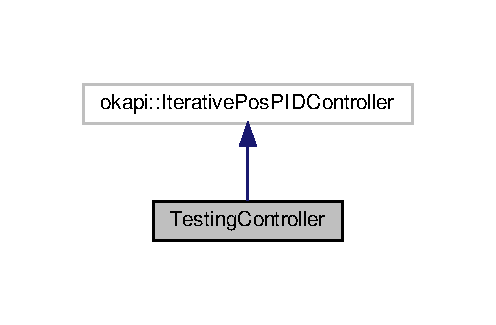
\includegraphics[width=238pt]{classTestingController__inherit__graph}
\end{center}
\end{figure}


Collaboration diagram for Testing\+Controller\+:\nopagebreak
\begin{figure}[H]
\begin{center}
\leavevmode
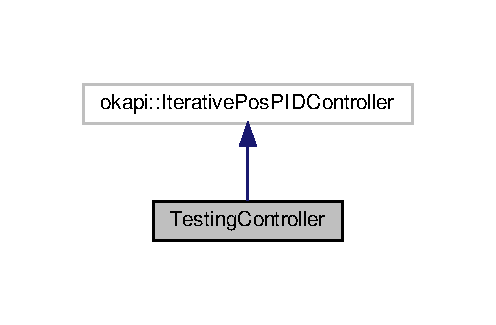
\includegraphics[width=238pt]{classTestingController__coll__graph}
\end{center}
\end{figure}
\subsection*{Public Member Functions}
\begin{DoxyCompactItemize}
\item 
\mbox{\Hypertarget{classTestingController_ab7cf58924cfe450061a9ac5967ff7a9f}\label{classTestingController_ab7cf58924cfe450061a9ac5967ff7a9f}} 
{\bfseries Testing\+Controller} (double ikP, double ikI, double ikD, double ik\+Bias, const okapi\+::\+Time\+Util \&itime\+Util, std\+::unique\+\_\+ptr$<$ okapi\+::\+Filter $>$ iderivative\+Filter=std\+::make\+\_\+unique$<$ okapi\+::\+Passthrough\+Filter $>$())
\item 
\mbox{\Hypertarget{classTestingController_acc6c9b4e7cbb485861d41864664cce6c}\label{classTestingController_acc6c9b4e7cbb485861d41864664cce6c}} 
double {\bfseries get\+Proportional\+Factor} ()
\item 
\mbox{\Hypertarget{classTestingController_a19a8ad24c637b49de618b8e0b4d07b8a}\label{classTestingController_a19a8ad24c637b49de618b8e0b4d07b8a}} 
double {\bfseries get\+Integral\+Factor} ()
\item 
\mbox{\Hypertarget{classTestingController_ada0e8d63e79dce67df2bc7896a69fb12}\label{classTestingController_ada0e8d63e79dce67df2bc7896a69fb12}} 
double {\bfseries get\+Derivative\+Factor} ()
\end{DoxyCompactItemize}


The documentation for this class was generated from the following file\+:\begin{DoxyCompactItemize}
\item 
src/pidtest.\+cpp\end{DoxyCompactItemize}

\hypertarget{structTrial}{}\section{Trial Struct Reference}
\label{structTrial}\index{Trial@{Trial}}


Collaboration diagram for Trial\+:\nopagebreak
\begin{figure}[H]
\begin{center}
\leavevmode
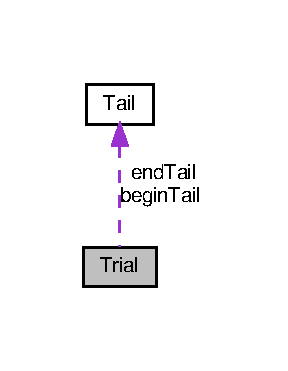
\includegraphics[width=138pt]{structTrial__coll__graph}
\end{center}
\end{figure}
\subsection*{Public Attributes}
\begin{DoxyCompactItemize}
\item 
\mbox{\Hypertarget{structTrial_aa03ccfb291ed9cc2b7078ae7e92d6891}\label{structTrial_aa03ccfb291ed9cc2b7078ae7e92d6891}} 
double {\bfseries d}
\item 
\mbox{\Hypertarget{structTrial_aebab47ba1a26683037a70407c1537a02}\label{structTrial_aebab47ba1a26683037a70407c1537a02}} 
double {\bfseries v}
\item 
\mbox{\Hypertarget{structTrial_a41622542930b88ee64929407e155e5a6}\label{structTrial_a41622542930b88ee64929407e155e5a6}} 
double {\bfseries a}
\item 
\mbox{\Hypertarget{structTrial_ab758b9fffe8a44d35ebc38212d973172}\label{structTrial_ab758b9fffe8a44d35ebc38212d973172}} 
double {\bfseries j}
\item 
\mbox{\Hypertarget{structTrial_a663812b290cd722ad79bab966a9157de}\label{structTrial_a663812b290cd722ad79bab966a9157de}} 
double {\bfseries kV}
\item 
\mbox{\Hypertarget{structTrial_a934b140a8aba892d5839afbf8689aa34}\label{structTrial_a934b140a8aba892d5839afbf8689aa34}} 
double {\bfseries kA}
\item 
\mbox{\Hypertarget{structTrial_a00912819027ccfa7755f4377ffcc2998}\label{structTrial_a00912819027ccfa7755f4377ffcc2998}} 
\hyperlink{structTail}{Tail} {\bfseries begin\+Tail}
\item 
\mbox{\Hypertarget{structTrial_a853567c8bf6d6459ae18ec56d311a71b}\label{structTrial_a853567c8bf6d6459ae18ec56d311a71b}} 
\hyperlink{structTail}{Tail} {\bfseries end\+Tail}
\item 
\mbox{\Hypertarget{structTrial_aacdc7ad201ec133e409338ff35e050e4}\label{structTrial_aacdc7ad201ec133e409338ff35e050e4}} 
bool {\bfseries stop\+On\+Finish}
\item 
\mbox{\Hypertarget{structTrial_aed31bb634a7e800e1b86e1039400da75}\label{structTrial_aed31bb634a7e800e1b86e1039400da75}} 
okapi\+::\+Abstract\+Motor\+::brake\+Mode {\bfseries stop\+Brake\+Mode}
\item 
\mbox{\Hypertarget{structTrial_a7c2901078783e3e51907100952730e7d}\label{structTrial_a7c2901078783e3e51907100952730e7d}} 
bool {\bfseries feedback\+On}
\end{DoxyCompactItemize}


The documentation for this struct was generated from the following file\+:\begin{DoxyCompactItemize}
\item 
src/followtest.\+cpp\end{DoxyCompactItemize}

\hypertarget{structTrialResults}{}\section{Trial\+Results Struct Reference}
\label{structTrialResults}\index{Trial\+Results@{Trial\+Results}}


Collaboration diagram for Trial\+Results\+:\nopagebreak
\begin{figure}[H]
\begin{center}
\leavevmode
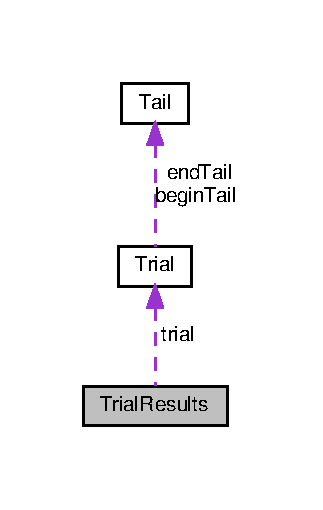
\includegraphics[width=155pt]{structTrialResults__coll__graph}
\end{center}
\end{figure}
\subsection*{Public Attributes}
\begin{DoxyCompactItemize}
\item 
\mbox{\Hypertarget{structTrialResults_a50b678689a2a82f47d8239de709374ce}\label{structTrialResults_a50b678689a2a82f47d8239de709374ce}} 
\hyperlink{structTrial}{Trial} {\bfseries trial}
\item 
\mbox{\Hypertarget{structTrialResults_a76e2d3fd3d323434445ee423ec94f957}\label{structTrialResults_a76e2d3fd3d323434445ee423ec94f957}} 
std\+::vector$<$ \hyperlink{structPosition}{Position} $>$ {\bfseries sampled\+Position}
\item 
\mbox{\Hypertarget{structTrialResults_a65f94af5cc330c857703220759c184dc}\label{structTrialResults_a65f94af5cc330c857703220759c184dc}} 
double {\bfseries final\+Velocity}
\end{DoxyCompactItemize}


The documentation for this struct was generated from the following file\+:\begin{DoxyCompactItemize}
\item 
src/followtest.\+cpp\end{DoxyCompactItemize}

%--- End generated contents ---

% Index
\backmatter
\newpage
\phantomsection
\clearemptydoublepage
\addcontentsline{toc}{chapter}{Index}
\printindex

\end{document}
